% Fig. 3: Three targets of distillation; representative methods follow the section taxonomy.
\begin{figure}[t]
\centering
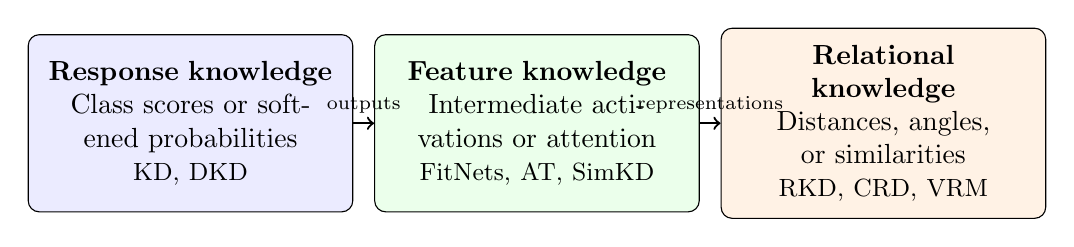
\begin{tikzpicture}[box/.style={draw,rounded corners,align=center,text width=3.7cm,minimum height=2.25cm,inner sep=6pt}, arr/.style={->,thick}]
\node[box,fill=blue!8] (response) {\textbf{Response knowledge}\\Class scores or softened probabilities\\\small KD, DKD};
\node[box,fill=green!8] (feature) at (4.4,0) {\textbf{Feature knowledge}\\Intermediate activations or attention\\\small FitNets, AT, SimKD};
\node[box,fill=orange!10] (relation) at (8.8,0) {\textbf{Relational knowledge}\\Distances, angles, or similarities\\\small RKD, CRD, VRM};
\draw[arr] (response) -- node[above,font=\scriptsize]{outputs} (feature);
\draw[arr] (feature) -- node[above,font=\scriptsize]{representations} (relation);
\end{tikzpicture}
\caption{Knowledge targets distinguish output responses, internal representations, and structure between examples. A method may combine targets; these categories describe its principal transferred signal.}
\label{fig:knowledge-types}
\end{figure}
